%& C:\Users\Nagaraj\AppData\Roaming\TikzEdt\TikzEdt\021~1.0\TEMP_H~1
\begin{document}

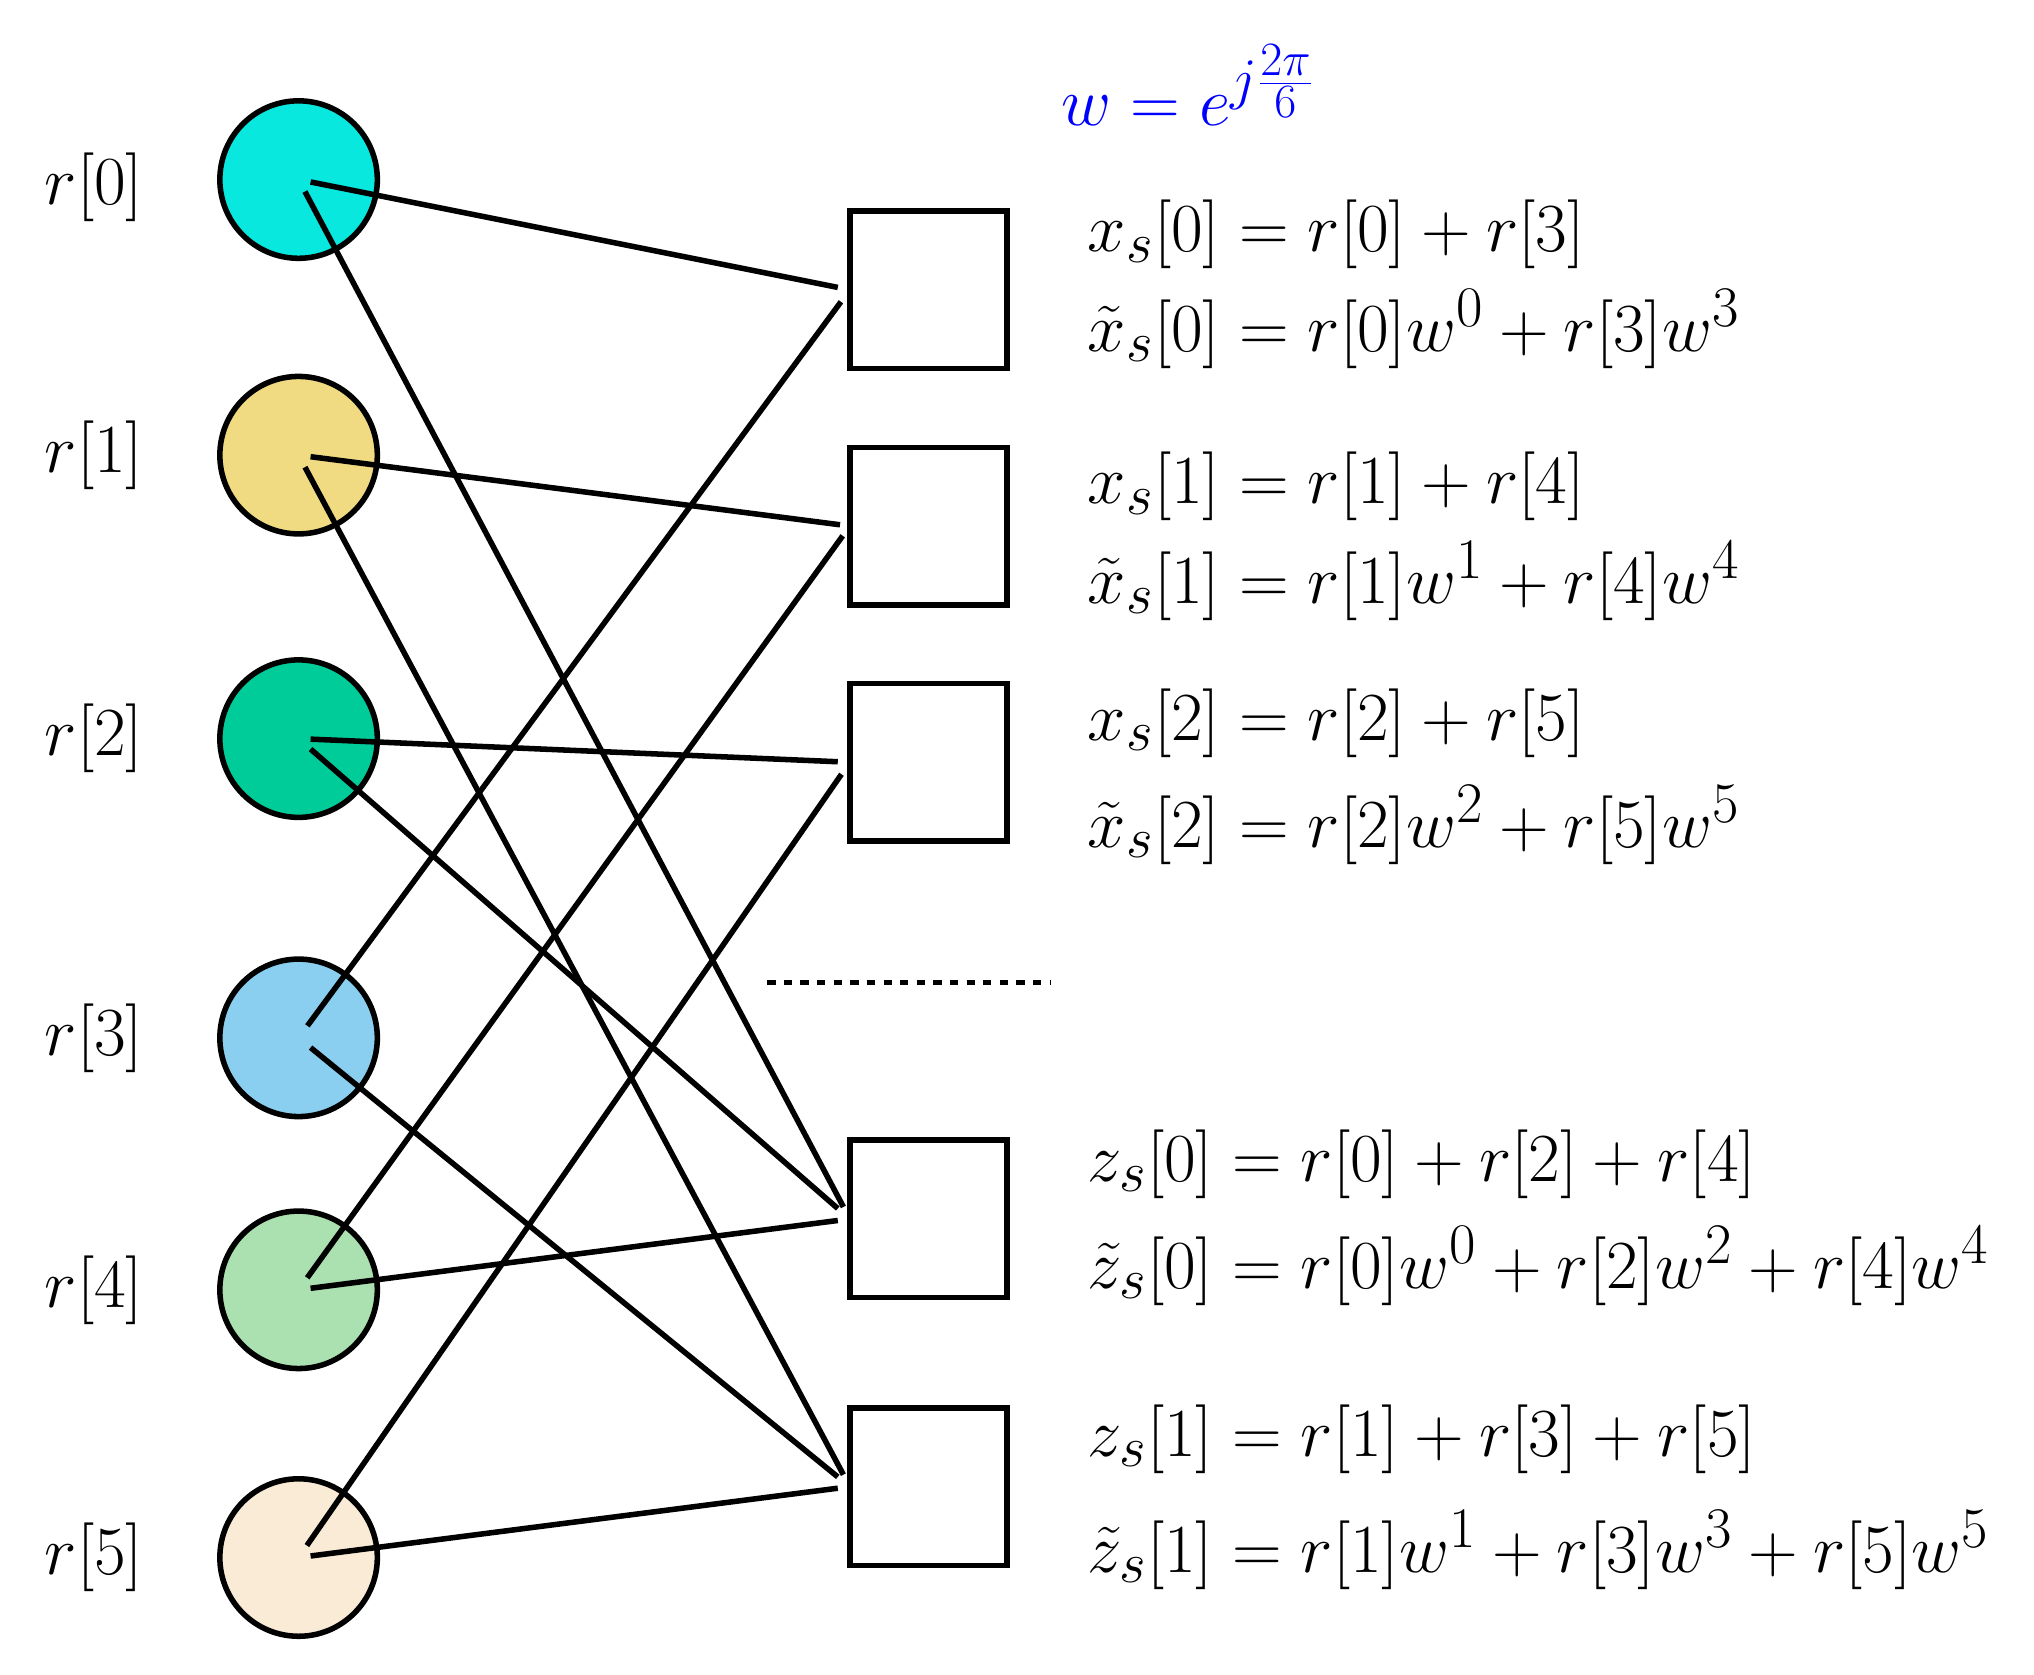
\begin{tikzpicture}

\definecolor{brightturquoise}{rgb}{0.03, 0.91, 0.87}
\definecolor{buff}{rgb}{0.94, 0.86, 0.51}
\definecolor{caribbeangreen}{rgb}{0.0, 0.8, 0.6}
\definecolor{celadon}{rgb}{0.67, 0.88, 0.69}
\definecolor{darktangerine}{rgb}{1.0, 0.66, 0.07}
\definecolor{darkviolet}{rgb}{0.58, 0.0, 0.83}
\definecolor{deepskyblue}{rgb}{0.0, 0.75, 1.0}
\definecolor{amber(sae/ece)}{rgb}{1.0, 0.49, 0.0}
\definecolor{antiquewhite}{rgb}{0.98, 0.92, 0.84}
\definecolor{applegreen}{rgb}{0.55, 0.71, 0.0}
\definecolor{babyblue}{rgb}{0.54, 0.81, 0.94}

% Variable nodes 
\draw [thick,fill=babyblue,line  width =2pt]   (-7,-6) node (v6) {} ellipse (1 and 1);
\draw[thick,fill=caribbeangreen,line  width =2pt]  (-7,-2.2) node (v5) {} ellipse (1 and 1);
\draw [thick,fill=buff,line  width =2pt]  (-7,1.4) node (v3) {} ellipse (1 and 1);
\draw  [thick,fill=celadon,line  width =2pt]  (-7,-9.2) node (v1) {} ellipse (1 and 1);
\draw  [thick,fill=antiquewhite,line  width =2pt]  (-7,-12.6) node (v1_1) {} ellipse (1 and 1);
\draw  [thick,fill=brightturquoise,line  width =2pt]  (-7,4.9) node (v1_2) {} ellipse (1 and 1);
%Check nodes


\draw [thick,line  width =2pt] (0,4.5) rectangle (2,2.5);
\draw [thick,line  width =2pt]  (0,1.5) node (v8) {} rectangle (2,-0.5);
\draw [thick,line  width =2pt] (0,-1.5) rectangle (2,-3.5);




\draw [thick,line  width =2pt] (0,-7.3) rectangle (2,-9.3);
\draw [thick,line  width =2pt] (0,-10.7) rectangle (2,-12.7);



\node at (-9.6,4.8) {\Huge $r[0]$};
\node at (-9.6,1.4) {\Huge $r[1]$};
\node at (-9.6,-2.2) {\Huge $r[2]$};
\node at (-9.6,-6) {\Huge $r[3]$};
\node at (-9.6,-9.2) {\Huge $r[4]$};
\node at (-9.6,-12.6) {\Huge $r[5]$};


\node [thick,line  width =2pt] (v2) at (0,3.5) {};
\node [thick,line  width =2pt] (v4) at (0,-2.5) {};


\node [thick,line  width =2pt] (v7) at (0,-8.3) {};
\node [thick,line  width =2pt] (v9) at (0,-11.7) {};

\node [thick,line  width =2pt] (v10) at (-1.2,-5.3) {};
\node [thick,line  width =2pt] (v11) at (2.7,-5.3) {};
\draw [thick,line  width =2pt][dashed] (v10) edge (v11);
\node [anchor=west] at (2.9,4.2) {\Huge $x_{s}[0] = r[0]+r[3]$};
\node [anchor=west] at (2.9,3) {\Huge $\tilde{x}_{s}[0] = r[0] w^{0}+r[3] w^{3}$};
\node [anchor=west] at (2.9,1) {\Huge $x_{s}[1] = r[1]+r[4]$};
\node [anchor=west] at (2.9,-0.2) {\Huge $\tilde{x}_{s}[1] = r[1] w^{1}+r[4] w^{4}$};
\node [anchor=west] at (2.9,-2) {\Huge $x_{s}[2] = r[2]+r[5]$};
\node [anchor=west] at (2.9,-3.3) {\Huge $\tilde{x}_{s}[2] = r[2] w^{2}+r[5] w^{5}$};

\node [anchor=west] at (2.9,-7.6) {\Huge $z_{s}[0] = r[0]+r[2]+r[4]$};
\node [anchor=west] at (2.9,-8.9) {\Huge $\tilde{z}_{s}[0] = r[0] w^{0}+r[2] w^{2}+r[4] w^{4}$};
\node [anchor=west] at (2.9,-11.1) {\Huge $z_{s}[1] = r[1]+r[3]+r[5]$};
\node [anchor=west] at (2.9,-12.5) {\Huge $\tilde{z}_{s}[1] = r[1] w^{1}+r[3] w^{3}+r[5] w^{5}$};

\draw [thick,line  width =2pt] (v1_2) edge (v2);
\draw [thick,line  width =2pt] (v1_2) edge (v7);

\draw [thick,line  width =2pt] (v3) edge (v9);
\draw [thick,line  width =2pt] (v5) edge (v4);
\node (v12) at (0,0.5) {};
\draw [thick,line  width =2pt] (v3) edge (v12);
\draw [thick,line  width =2pt] (v5) edge (v7);

\draw [thick,line  width =2pt] (v6) edge (v2);
\draw [thick,line  width =2pt](v1) edge (v12);
\draw [thick,line  width =2pt] (v1_1) edge (v4);
\draw [thick,line  width =2pt] (v6) edge (v9);
\draw [thick,line  width =2pt] (v1_1) edge (v9);
\draw [thick,line  width =2pt] (v1) edge (v7);
\node at (4.3,6.1) {\color{blue} \Huge$w=e^{j \frac{2\pi}{6} }$};

\usetikzlibrary{calc}
\pgftransformreset
\node[inner sep=0pt,outer sep=0pt,minimum size=0pt,line width=0pt,text width=0pt,text height=0pt] at (current bounding box) {};
%add border to avoid cropping by pdflibnet
\foreach \border in {0.1}
  \useasboundingbox (current bounding box.south west)+(-\border,-\border) rectangle (current bounding box.north east)+(\border,\border);
\newwrite\metadatafile
\immediate\openout\metadatafile=\jobname_BB.txt
\path
  let
    \p1=(current bounding box.south west),
    \p2=(current bounding box.north east)
  in
  node[inner sep=0pt,outer sep=0pt,minimum size=0pt,line width=0pt,text width=0pt,text height=0pt,draw=white] at (current bounding box) {
\immediate\write\metadatafile{\p1,\p2}
};
\immediate\closeout\metadatafile
\end{tikzpicture}

\end{document}

